\documentclass[10pt]{article}
\usepackage{blindtext}
\usepackage[total={7in, 9in}]{geometry}
\usepackage[utf8]{inputenc}
\usepackage{graphicx}
\usepackage{amsmath}
\usepackage{amsfonts}
\usepackage{amssymb}

% Title Page
\title{E102 Final Report}
\author{Pierce Gruber, Kaitlin Lucio}


\begin{document}
\maketitle

\begin{abstract}
Moving a cart with an inverted pendulum is an inherently tricky system as it requires both disturbing and maintaining an unstable equilibrium to move the cart to a desired location. One method to solve this problem is using a state-space system in feedback to calculate the needed acceleration vector using an observer to correct for non-linearities in the system. In doing so, the pendulum may be maintained as upright while still moving the cart according to a desired position without overshoot. This report describes one such process and solution for such a system using MATLAB.
\end{abstract}

\section{Problem Statement}
A cart with an inverted pendulum of length $L = 0.5\text{ m}$ and a max acceleration of $|\text{a}(t)| < 0.5 \text{ m}/\text{sec}^2$ and is subject to an angular acceleration disturbance $\alpha(t) = 0.5$ rad$/\text{sec}^{2}$. The cart must move to a final displacement from its starting location of $10$ m within an overall time limit of $10$ seconds without overshooting its target.

The cart is able to measure its displacement $s(t)$ and its current pendulum angle $\theta(t)$.

\begin{center}
    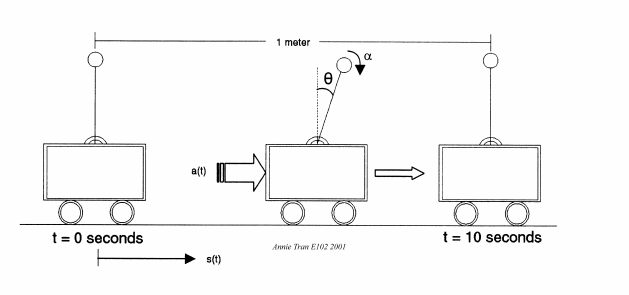
\includegraphics{graphs/invpen.png}
\end{center}

The governing equations for this system are given by the following

\begin{align*}
    L\frac{d^{2}\theta}{dt^{2}} &- g\text{sin}(\theta(t)) = -a(t)\text{cos}(\theta(t)) + L\alpha(t) \\
    \frac{d^2s}{dt^2} &= a(t)
\end{align*}

Rearranging yields the following governing equations

\begin{align*}
    \frac{d^{2}\theta}{dt^{2}} &= \frac{g}{L}\text{sin}(\theta(t)) - \frac{1}{L}a(t)\text{cos}(\theta(t)) + \alpha(t) \\
    \frac{d^2s}{dt^2} &= a(t)
\end{align*}

and for a state-space set of equations, we must linearize this. Using $\text{sin}(\theta) = \theta$ and $\text{cos}(\theta) = 1$, we get

\begin{align*}
    \frac{d^{2}\theta}{dt^{2}} &= \frac{g}{L}\theta - \frac{1}{L}a(t) + \alpha(t) \\
    \frac{d^2s}{dt^2} &= a(t)
\end{align*}

Given state vector $\bar{x} = \begin{bmatrix} \theta \\ \dot{\theta} \\ s \\ \dot{s} \end{bmatrix}$ and control input $u = a(t)$, a disturbance $\omega = \alpha(t)$, and an output vector $\bar{y} = \begin{bmatrix} \theta \\ s \end{bmatrix}$, we can write out a set of matrices for this system when not in any sort of feedback. This results in the following matrices for the state space equations $\dot{\bar{x}} = A\bar{x} + Bu$ and $\bar{y} = C\bar{x} + Du$. Note that our $\bar{x}$ implies $\dot{\bar{x}} = \begin{bmatrix} \dot{\theta} \\ \ddot{\theta} \\ \dot{s} \\ \ddot{s} \end{bmatrix}$

\begin{center}
    \begin{tabular}{| c | c |}
        \hline
        A & $\begin{bmatrix}
                0 & 1 & 0 & 0 \\
                \frac{g}{L} & 0 & 0 & 0 \\
                0 & 0 & 0 & 1 \\
                0 & 0 & 0 & 0
             \end{bmatrix}$ \\
        \hline
        B & $\begin{bmatrix}
                0 & -\frac{1}{L} & 0 & 1
             \end{bmatrix}$ \\
        \hline
        C & $\begin{bmatrix}
                1 & 0 & 0 & 0 \\
                0 & 0 & 1 & 0
             \end{bmatrix}$ \\
        \hline
        D & $\begin{bmatrix}
                0
             \end{bmatrix}$ \\
        \hline
    \end{tabular}
\end{center}

where we ignore the disturbance $\alpha(t)$.

We note that for our system as described above, we can calculate $M_c$ and $M_o$. This results in the following matrices.

\begin{center}
    \begin{tabular}{| c | c |}
        \hline
        $M_c$ & $\begin{bmatrix}
                0 & -2 & 0 & -39.2 \\
                -2 & 0 & -39.2 & 0 \\
                0 & 1 & 0 & 0 \\
                1 & 0 & 0 & 0
             \end{bmatrix}$ \\
        \hline
        $M_o$ & $\begin{bmatrix}
                1 & 0 & 0 & 0 \\
                0 & 0 & 1 & 0 \\
                0 & 1 & 0 & 0 \\
                0 & 0 & 0 & 1
             \end{bmatrix}$ \\
        \hline
    \end{tabular}
\end{center}

which are both invertible and thus the system is both invertible and controllable.

\end{document}
